
%%%%%%%%%%%%%%%%%%%%%%%%%%%%%%% INTRO %%%%%%%%%%%%%%%%%%%%%%%%%%%%%

%We attach unique identifiers to type holes, interpret them as type variables, and infer types for holes with Hindley-Milner \emph{type inference} \cite{MilnerInfer} based on unification \cite{RobinUnification}. The algorithm follows two standard steps, constraint generation and constraint solving by unification.

%The implementation inserts holes automatically, following the \Hazelnut edit action calculus, to guarantee that every editor state has some (possibly incomplete) type.

\section{Type Hole Inference}
\subsection{Introduction}
\label{sec:intro}
%%%%%%%%%%%%%%%%%%%%%% INTRO TODOS %%%%%%%%%%%%%%%%%%%%%%

\todo{LATER: Make this into a "mini paper"}

\emph{Bidirectional typing} and \emph{constraint-based type inference} are common approaches to deducing types for partially annotated programs. 
%\emph{Bidirectional typing} is a simple algorithmic system with type information propagating from the outside in \cite{BidirTyping}. 
This produces clear error messages at the cost of requiring explicit type annotations in certain situations, e.g. top-level functions. \emph{Type inference} allows programmers to omit most or all type annotations, but requires complex constraint solving for type checking, making it difficult for users to reason about types and producing complex error messages \cite{typeinferDif}.
This paper develops \emph{type hole inference}, which combines the benefits of bidirectional typing and type inference.\par

In recent work on the \Hazel programming environment, \citet{HazelnutPOPL} assign formal meaning to incomplete programs, i.e. programs with holes, by developing a bidirectional type system with support for expression and type holes. Type holes operate as the unknown types from gradual type theory \cite{GradualTyping}. Our approach takes this type system and adds constraint solving as a layer on top to suggest type hole fillings, without making constraint solving necessary for typing. 

We define "solving" the constraints associated with a given type hole as the process of (1) identifying all of its possible type substitutions and (2) reporting the most informative substitutions to the user. If all possible substitutions are consistent with each other and do not elicit occurs check failure, the type hole is deemed \emph{solvable}.

\emph{Type hole inference} takes two steps: (1) use bidirectional typing for type checking, type synthesis and constraint generation; (2) solve the constraint set to infer types for type holes. In contrast to \emph{type inference}, our approach has the following features: (1) we separate type checking and constraint solving into two steps. The system only does type checking and triggers static errors at the first step; (2) expressions remain well-typed when the constraint solver can not find a solution for type variables, for instance when one type variable is equal to multiple types. The system postpones the remaining type checking to runtime. Since  type variables may be unconstrained after unification, we can generalize those type holes by introducing polymorphism in the future work. 

Through the constraint solving layer of \emph{Type Hole Inference}, the user is given suggestions for type holes which are \textit{solvable}. In addition, \emph{type hole inference} provides debug information for \emph{unsolvable} type holes by presenting a \emph{PotentialTypeSet} containing all possible substitutions. When the user selects an \emph{unsolvable} type hole, rather than blaming one particular expression, the editor highlights the origins of all types that rendered it \emph{unsolvable}. Error localization feedback is visual and updated as edits occur, allowing the user to interactively repair their program.

\par{Contributions} The contributions of this paper are: (1) a new bidirectional typing system extended with type constraints in section ~\ref{sec:typinf}; (2) a type inference algorithm to handle type holes in section without failure upon hitting unsolvable constraints ~\ref{sec:infalg}.

\subsection{User Interaction}

Taking advantage of the interactiveness of live programming, rather than guessing sources of blame, we simply ask the user. \emph{Type hole inference} displays all possible sources of inconsistency and allows the user to identify which to blame. Once a user attempts to fix the program, the editor can display new errors as they arise. In this manner, the program can be iteratively and interactively repaired. 

Take the following \Hazel programs extended with type hole inference as examples: 

\begin{figure}[h!]
\centering
  \begin{tabular}[b]{cc}
    \begin{tabular}[b]{c}
      \begin{subfigure}[b]{0.4\columnwidth}
        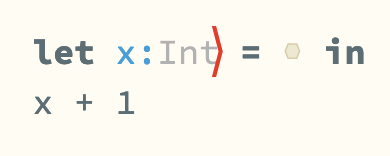
\includegraphics[width=5.5cm]{images/haz3l-ghost}
        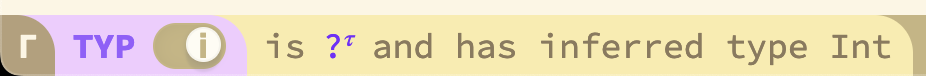
\includegraphics[width=5.5cm]{images/haz3l-ghost-inferred-type.png}
        \caption{constraint solving success}
        \label{fig:inference_success_ghost}
      \end{subfigure}\\
      \begin{subfigure}[b]{0.4\columnwidth}
              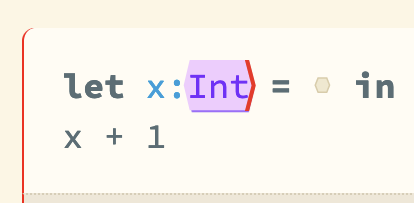
\includegraphics[width=5.5cm]{images/haz3l-accepted-ghost.png}
            \caption{user accepts suggested type annotation}
    		\label{fig:inference_success_accept_suggestion}
      \end{subfigure}
    \end{tabular}
    &
     \begin{tabular}[b]{c}
    \begin{subfigure}[b]{0.4\columnwidth}
        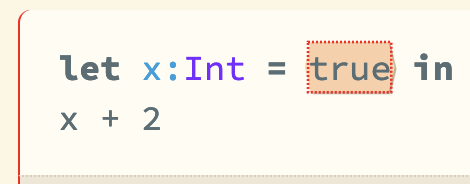
\includegraphics[width=5.5cm]{images/haz3l-static-error}
        \caption{user fills expression hole with true}
        \label{fig:static_error}
    \end{subfigure}\\
      \begin{subfigure}[b]{0.4\columnwidth}
            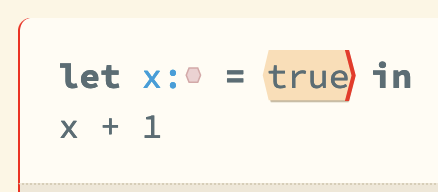
\includegraphics[width=5.5cm]{images/haz3l-red-grout}
            
\includegraphics[width=5.5cm]{images/haz3l-red-grout-type-set.png}
            \caption{user deletes type annotation}
            \label{fig:inference_error}
      \end{subfigure}
    \end{tabular}
  \end{tabular}
  \caption{Programs in Hazel environment}
  \vspace{-2px}
\end{figure}
\par Figure ~\ref{fig:static_error} illustrates Hazel's bidirectional type system catching a static error then wrapping the expression in a non-empty hole. The editor indicates the error's source with a red box, showing that the operand should be $Int$ type. \par

Figure ~\ref{fig:inference_error} shows a program that fails constraint solving, because the constraints $(\tehole^p \approx Int)$ and $(\tehole^p ~ \approx ~ Bool)$ conflict, where $\tehole^p$ is an unknown type hole variable for variable $x$. In this example, the error is localized to the type annotation for variable $x$. In the editor's Cursor Inspector, \textbf{all possible types}, given the constraints, for the variable $x$'s annotation are listed to aid the user in discerning the intended type for $x$.

Figure ~\ref{fig:inference_success_ghost} is an example succeeding in both static checking and constraint solving.  The constraint solver can infer that variable $x$ must be an integer, because it is the left operand of the plus $+$ operator. Hence, the type hole is filled with a gray "$Int$" in the editor. The programmer can hit the Enter key to replace the type hole with the suggested type as shown in Figure ~\ref{fig:inference_success_accept_suggestion}, and the expression is synthesized to "$\tarr{Int}{Int}$" after replacement. \par

%%%%%%%%%%%%%%%%%%%%%%%%%%%%%%% TYPE SYSTEM %%%%%%%%%%%%%%%%%%%%%%%%%%%%%

\subsection{Type System}

\label{sec:typinf}
Figure ~\ref{fig:syntax_fig} defines the syntax of H-types and H-expressions. We start from the definition given in \citet{HazelnutPOPL} except two modifications. First, we add an annotated lambda. Second, we attach a unique \emph{type hole provenance}, drawn as a superscript lower case letter, to each type hole, such as $\tehole^p$. Type holes are unknown type variables, and must be differentiated from one another during constraint generation and constraint solving. There are two types of expression holes: empty holes, $\ehole^n$, standing for missing parts of an incomplete program, and non-empty holes, $\notehole{e}^n$, operating as membranes around static and dynamic type inconsistencies \cite{HazelLive}. Both types of expression holes are uniquely identified by an integer id $n$. \par
\begin{figure}[h!]
\vspace{-3px} 
$\arraycolsep=4pt\begin{array}{lll}
HProv~~ p & ::= & 
    n ~\vert~ 
    \rightarrow_{L}(p) ~\vert~ 
    \rightarrow_{R}(p)
    \\
HTyp~~ \tau & ::= &
  \tnum ~\vert~
  \tbool ~\vert~
  \tarr{\tau}{\tau} ~\vert~
  \tehole^p
  \\
HExp~~ e & ::= &
  x ~\vert~
  \lamfunc{x}{e} ~\vert~
  \lamfunc{x:\tau}{e} ~\vert~
  e(e) ~\vert~
  \underlinenum{n} ~\vert~
  (e+e) ~\vert~
  e: \tau ~\vert~
  \ehole^{n}  ~\vert~
  \notehole{e} 
\end{array}$
\hrule
\caption{Syntax of H-types, H-expressions, and Type Constraint Set}
\label{fig:syntax_fig}
\vspace{-5px}
\end{figure}

\subsection{Constraint Generation}
\todo{this section assumes eholes have ids; edit section above to permit this}
Central to any type inference system is constraint generation. This topic has been widely explored in literature and is commonly completed alongside type checking (citation needed \todo{cite tapl and expand slightly}). We approach constraint generation from a notion of enforcing our expectations of various expressions and their types as we perform synthesis and analysis. Constraints can be accumulated across uses of bidirectional typing judgements after expression marking to generate a final set of constraints. To facilitate this, we extend our previous judgement forms for the synthesis and analysis of matched expressions as follows:
$$\ctxSynType{\ctx}{\ECMV}{\TMV} ~|~ C$$ 
$$\ctxAnaType{\ctx}{\ECMV}{\TMV} ~|~ C$$
Here, the set of constraints the judgement occurs under is captured in $C$.

In some sense, the set of constraints $C$ represents all expected consistencies in a program. One key mechanism by which we facilitate our accumulation of expectations is analysis. Indeed, when we expect something should have a type \TMV, we commonly analyze it against that type. As a classic example of this let us explore subsumption. In situations where we expect a subsumable marked expression to analyze against a type $\tau$, the type $\tau'$ it synthesizes to is expected to be consistent with the input. This is checked with a premise assessing consistency. In order to more concretely track this as a constraint, we extend the rule MASubsume \todo{fix styling on rule names so its consistent with Eric's} as follows:

\begin{mathpar}
  \judgment{
    \ctxSynType{\ctx}{\ECMV}{\TMV'} ~|~ C \\
    \consistent{\TMV}{\TMV'} \\
    \subsumable{\ECMV}
  }{
    \ctxAnaType{\ctx}{\ECMV}{\TMV} ~|~ C \cup \{ \TMV \approx \TMV' \}
  }{MASubsume-C}
\end{mathpar}

Here, we concretize out expectation of $\tau ~ \tau'$ by generating a new constraint: $\tau \approx \tau'$. Additionally, we accumulate constraints generated in each premise in our conclusion

However, one key question is how we manage constraints whenever marked expressions are wrapped in holes. Should expectations of types pass through the hole membrane and render expressions inside unsolved? On a similar tack, should a program inside some hole membrane seep out and affect the rest of the program? We assert that the answer to both of these questions is no. Nonempty holes act as quarantines that allow the programmer to reason as if expressions inside them are unaffected by and do not affect the program around them.

With this guiding principle in hand, let us approach constraint generation for subsumption when the argument of analysis $\tau$ is different from the result of synthesis $\tau'$ by extending MAInconsistentTypes:

\begin{mathpar}
  \judgment{
    \ctxSynType{\ctx}{\ECMV}{\TMV'} ~|~ C  \\
    \inconsistent{\TMV}{\TMV'} \\\\
    \subsumable{\ECMV}
  }{
    \ctxAnaType{\ctx}{\ECInconType{\ECMV}^n}{\TMV} ~|~ C \cup \{ \TMV \approx \tehole^n \}
  }{MAInconsistentTypes-C}
\end{mathpar}

Here we accumulate constraints from our premises just as before. However, instead of expecting that the type of \ECMV~ be the consistent with the type $\tau$ when this is clearly impossible, we prevent the external conflict from $\tau$ reaching beyond our type hole. Rather we enforce that the hole surrounding \ECMV~ synthesize a type consistent with $\tau$.

Expectations for the result of typechecking on expressions is not limited to analysis. Indeed, there are multiple cases where we hold expectations for the types of our expressions in synthesis as well. As a simple example, consider if expressions. We expect that branches have consistent types, and assess this implicitly by attempting to compute their lower bound. This leads to the following constraint generating rule for if expression synthesis:

\begin{mathpar}
  \judgment{
    \ctxAnaType{\ctx}{\ECMV_1}{\TBool} ~|~ C_1  \\\\
    \ctxSynType{\ctx}{\ECMV_2}{\TMV_1} ~|~ C_2 \\
    \ctxSynType{\ctx}{\ECMV_3}{\TMV_2} ~|~ C_3
  }{
    \ctxSynType{\ctx}{\ECIf{\ECMV_1}{\ECMV_2}{\ECMV_3}}{\TJoin{\TMV_1}{\TMV_2}} ~|~ C_1 \cup C_2 \cup C_3 \cup \{ \TMV_1 \approx \TMV_2 \}
  }{MSIf-C}
\end{mathpar}

Here, we simply accumulate constraints and require that $\TMV_1 \approx \TMV_2$. 

Our logic for when the branches of an if expression have no lower bound is somewhat trickier, but follows the same logic as before. Inconsistency among branches can be considered an error that lies within the hole surrounding our marked expression. Consequently, we can constrain $\TMV_1 \approx \TMV_2$ as before:

\begin{mathpar}
  \judgment{
    \ctxAnaType{\ctx}{\ECMV_1}{\TBool} ~|~ C_1 \\
    \ctxSynType{\ctx}{\ECMV_2}{\TMV_1} ~|~ C_2 \\\\
    \ctxSynType{\ctx}{\ECMV_3}{\TMV_2} ~|~ C_3 \\
    \inconsistent{\TMV_1}{\TMV_2}
  }{
    \ctxSynType{\ctx}{\ECInconBr{\ECMV_1}{\ECMV_2}{\ECMV_3}}{\TUnknown} ~|~ C_1 \cup C_2 \cup C_3 \cup \{ \TMV_1 \approx \TMV_2 \}
  }{MSInconsistentBranches-C}
\end{mathpar}

How might we approach lambdas or the application of lambdas? While the procedure for approaching these types of is much the same as those we've discussed, before defining new rules for them we must adjust our definition of the matched arrow judgement. 

When we generate a matched arrow form for a type hole, we are expecting that the original type hole be equal to the arrow type outputted by the judgement. This straightforward constraint can be represented as follows:

\begin{mathpar}
\judgment{ }{
  \matchedArrow{\TUnknown^p}{\TUnknown^{\rightarrow_L(p)}}{\TUnknown^{\rightarrow_R(p)}} ~|~ \{ \TUnknown^p \approx \tarr{\TUnknown^{\rightarrow_L(p)}}{\TUnknown^{\rightarrow_R(p)}} \}
}{TMAHole-C}
\end{mathpar}

With this new definition of matched arrow in hand, we can approach lambdas and their application. When synthesizing the type of an annotated lambda expression, we don't exert any expectation on the results of synthesis. This leads to this straightforward extension of our previous synthesis rule:

\begin{mathpar}
    \judgment{
        \ctxSynType{\extendCtx{\ctx}{x}{\TMV}}{\ECMV}{\TMV_2} ~|~ C
    }{
        \ctxSynType{\ctx}{\ECLam{x}{\TMV_1}{\ECMV}}{\TArrow{\TMV_1}{\TMV_2}} ~|~ C
    }{MSLam-C}
\end{mathpar}

Our rule for analysis of annotated lambdas when no local errors are present is similar, but encodes one key difference. Here, we assert that the annotation \TMV be consistent with the input type of the argument to analysis:

\begin{mathpar}
  \judgment{
    \matchedArrow{\TMV_3}{\TMV_1}{\TMV_2} ~|~ C_1\\
    \consistent{\TMV}{\TMV_1} \\\\
    \ctxAnaType{\extendCtx{\ctx}{x}{\TMV}}{\ECMV}{\TMV_2} ~|~ C_2
  }{
    \ctxAnaType{\ctx}{\ECLam{x}{\TMV}{\ECMV}}{\TMV_3} ~|~ C_1 \cup C_2 \cup \{ \TMV \approx \TMV_1 \}
  }{MALam1-C}
\end{mathpar}

Our rules for the remaining two lambda analysis cases where the lambda expression is wrapped in a hole are trickier. Let us begin by assessing the case where the analyzed type has no matched arrow form. In such cases, we previously analyzed the body of the lambda against the unknown type to ensure its validity \todo{ask why we do this}. However, which unknown type are we analyzing the body against? As discussed earlier, performing analysis imparts the expectation that the type of the expression is consistent with the argument of analysis. If we were to simply analyze against the type of the hole membrane we use to surround the marked lambda, we'd impart the expectation that the inside of the lambda be consistent with the hole itself. This would subvert our goal of separating the program outside the hole with that inside! In fact, any hole we choose would impart some invalid expectation with respect to the goals we've outlined. Consequently, we introduce the anonymous type hole: this type hole is represented by the provenance $anon$ and will have its constraints ignored by the constraint solver when we later explore unification.

\begin{center}
    $\arraycolsep=4pt\begin{array}{lll}
    HProv~~ p & ::= & 
        ... ~\vert~ 
        anon
        \\
    \end{array}$
\end{center}

Using this type hole, we can analyze the lambda's body against an unknown type without linking it spuriously to some other type hole:

\begin{mathpar}
  \judgment{
    \notMatchedArrow{\TMV_3} \\
    \ctxAnaType{\extendCtx{\ctx}{x}{\TMV}}{\ECMV}{\TUnknown^{anon}} ~|~ C
  }{
    \ctxAnaType{\ctx}{\ECInconType{\ECLam{x}{\TMV}{\ECMV}}}{\TMV_3} ~|~ C \cup \{ \TUnknown^{n} \approx \TMV_3 \}
  }{MALam2-C}
\end{mathpar}

Note that the conclusion of this rule adds the constraint $\{ \TUnknown^{n} \approx \TMV_3 \}$. The argument of analysis $\TMV_3$ constitutes an expectation of types from outside the hole surrounding our lambda. Consequently, rather than allowing it to influence the program inside the hole, we simply constrain $\TMV_3$ to the hole's type $?^n$.

The rule for analysis of annotated lambdas when the our annotation is inconsistent with the input type of our analyzed type is similarly defined:

\begin{mathpar}
  \judgment{
    \matchedArrow{\TMV_3}{\TMV_1}{\TMV_2} ~|~ C_1\\
    \inconsistent{\TMV}{\TMV_1} \\\\
    \ctxAnaType{\extendCtx{\ctx}{x}{\TMV}}{\ECMV}{\TMV_2} ~|~ C_2
  }{
    \ctxAnaType{\ctx}{\ECInconType{\ECLam{x}{\TMV}{\ECMV}}}{\TMV_3} ~|~ C_1 \cup C_2 \cup \{ \TUnknown^{n} \approx \TMV_3 \}
  }{MALam3-C}
\end{mathpar}

This brings us at last to synthesis for the application of lambdas. When the function position expression has a matched arrow form, our rule simply needs to accumulate the constraints of its premises:

\begin{mathpar}
  \judgment{
    \ctxSynType{\ctx}{\ECMV_1}{\TMV} ~|~ C_1 \\
    \matchedArrow{\TMV}{\TMV_1}{\TMV_2} ~|~ C_2 \\\\
    \ctxAnaType{\ctx}{\ECMV_2}{\TMV_1} ~|~ C_3
  }{
    \ctxSynType{\ctx}{\ECAp{\ECMV_1}{\ECMV_2}}{\TMV_2} ~|~ C_1 \cup C_2 \cup C_3
  }{MSAp1-C}
\end{mathpar}

When the function position expression lacks a match arrow form, we wrap it in a marked expression hole and proceed as if we had called matched arrow on the hole. To facilitate this, the argument expression must be analyzed against $\TUnknown^{\rightarrow_L{n}}$ and we must return $\TUnknown^{\rightarrow_R{n}}$ as the result of synthesis. 


\begin{mathpar}
  \judgment{
    \ctxSynType{\ctx}{\ECMV_1}{\TMV} ~|~ C_1 \\
    \notMatchedArrow{\TMV} \\\\
    \ctxAnaType{\ctx}{\ECMV_2}{\TUnknown} ~|~ C_2
  }{
    \ctxSynType{\ctx}{\ECApNonMatchedAltAlt{\ECMV_1}{\ECMV_2}}{\TUnknown} ~|~ C_1 \cup C_2 \cup \{ \TUnknown^n \approx \tarr{\TUnknown^{\rightarrow_L(n)}}{\TUnknown^{\rightarrow_R(n)}}\}
  }{MSAp2'-C}
\end{mathpar}

The remaining rules are all the same as their non constraint generating counterparts, except that they accumulate constraints from each of their premises as done above. As a result, they are somewhat repetitive and are consequently left to our supplementary material in Appendix B \todo{How exactly do we put this in supplementary material and do we actually wanna do that?}.
  
We leverage Hazel's type system to generate constraints inductively through bidirectional propagation. Figure ~\ref{fig:ana-syn} defines a bidirectional typing system extended with type constraint sets. A \emph{type constraint set} is written as $C$. The typing context, $\Gamma$, maps a set of expression variables to their types. Rule ~\ref{rule:syn-ehole} and ~\ref{rule:syn-hole} synthesize an expression hole to hole type. Rule ~\ref{rule:ana-subsume} and ~\ref{rule:ana-lam} have type consistency in their premises, generating new constraints and merging them into constraint sets in the conclusion. Rule ~\ref{rule:syn-ap}, ~\ref{rule:ana-lam} and ~\ref{rule:ana-lamann} have \emph{matched arrow type judgements} defined in figure ~\ref{fig:match-arrow-typ}. They leave the arrow type unchanged and assign the type hole the matched arrow type $\tarr{\tehole^{\rightarrow_{L}(p)}}{\tehole^{\rightarrow_{R}(p)}}$ where new holes are uniquely identified by matched arrow provenances generated from the original hole $\tehole^{p}$ and constraint generation links the original hole to its matched counterpart \cite{HazelnutPOPL}.

% 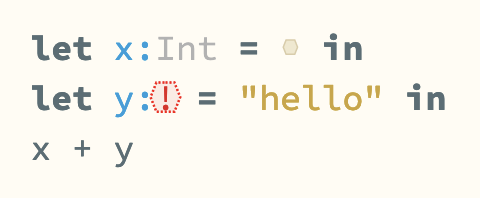
\includegraphics[width=5.5cm]{images/constraint_gen_example2.png}

\todo{add an example of a correct program for constraint generation}
\todo{add a setence explaining that a lot of the bidirectional typing rules don't add constraints, just recursively gather them from subexpressions and propogate them further}
\todo{add a typing rule for let since it's used in examples}
\todo{condense transitivity discussion}
We use the symbol $\approx$ to represent the constraint relation where if $\tau_1 \approx \tau_2$, $\tau_1$ and $\tau_2$ are \textit{allegedly} the same type, and share the same solution. We refrain from using $=$ because, to our constraint solver, the relation is not transitive. 
For example, consider the constraint set $C_{ex1} = \{ \tehole^{1} \approx \tnum, ~ \tnum \approx~ \tehole^{2}\}$. Even though $\tehole^{1}$ and $\tehole^{2}$ are both constrained to $\tnum$, the constraint solver would not consider $\tehole^{1}$ and $\tehole^{2}$ to have the same solution. To make this more concrete, consider the following program:
\begin{center}
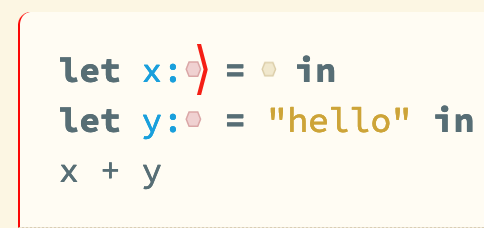
\includegraphics[width=5cm]{images/constraint_gen_bad_example.png}
\end{center}
Here, $\tehole^{x} \approx \tnum$ and $\tehole^{y} \approx \tnum$ because they are operands of the plus $+$ operator, and $\tehole^{y} \approx String$ because it is bound to $"hello"$. If the constraint relation were always transitive, $\tehole^x$ would be considered to have the same solution as $\tehole^y$, because $x$ and $y$ are both constrained to $Int$! This is undesirable, because ideally $x$ should be solved to have type $Int$ even if $y$ has conflicting constraints to $Int$ and $String$. If the constraint relation were to be transitive, both $x$ and $y$ would be unsolved.
Alternatively, in the example below, $x$ is not considered to have the same solution as $y$, and so although $y$ is unsolved due to conflicting constraints $Int$ and $String$, x is solved to $Int$:
\begin{center}
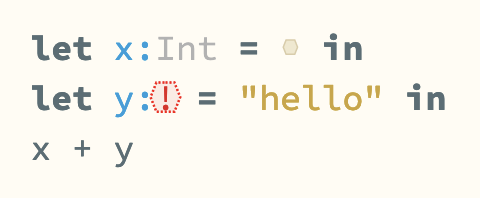
\includegraphics[width=5cm]{images/constraint_gen_example2.png}
\end{center}

% \begin{figure}[b]
%     \centering
%     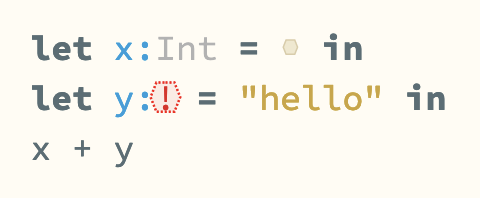
\includegraphics[width=5cm]{images/constraint_gen_example2.png}
%     \caption{An editor that does not constrain x to y}
%     \label{fig:IntransitiveEx2}
% \end{figure}

Additionally, the constraint relation $\approx$ is distinct from the consistency relation $\sim$. As an example, consider the constraint set $C_{ex2} = \{ \tehole^{1} \approx \tnum, ~ \tehole^{1} \approx~ \tehole^{2}\}$. Here, knowing that $\tehole^{1} \approx \tnum$ and $\tehole^{1} \approx \tehole^{2}$, our constraint solver would infer that $\tehole^{2} \approx \tnum$. On the other hand, given only the consistency relations $\{ \tehole^{1} \sim \tnum, ~ \tehole^{1} \sim~ \tehole^{2}\}$, it cannot be concluded that $ \tehole^{2} \sim \tnum$.

% \begin{figure}[h!]
% \vspace{-3px} 
%     \begin{multicols}{2}
%       \fbox{$\consexptyp{\Gamma}{e}{\tau}{C}$}~~\text{$e$ synthesizes $\tau$}\hfill
%     \begin{subequations}
%     \begin{equation}\label{rule:syn-var}
%         \inferrule[]{ }{
%             \consexptyp{\Gamma, x : \tau}{x}{\tau}{\econs}
%           }
%     \end{equation}
%     \begin{equation}\label{rule:syn-num}
%         \inferrule[]{ }{
%             \consexptyp{\Gamma}{\hnum{n}}{\tnum}{\econs}
%           }
%     \end{equation}
%     \begin{equation}\label{rule:syn-plus}
%         \inferrule[]{
%             \ana{\Gamma}{e_1}{\tnum}{C_1} \\
%             \ana{\Gamma}{e_2}{\tnum}{C_2}
%           }{
%             \consexptyp{\Gamma}{(e_1 + e_2)}{\tnum}{C_1 \cup C_2}
%           }
%     \end{equation}
%     \begin{equation}
%         \inferrule[]{
%             \ananc{\Gamma}{e_1}{\tnum}\\
%             \ananc{\Gamma}{e_2}{\tnum}
%           }{
%             \consexptypnc{\Gamma}{(e_1 + e_2)}{\tnum}
%           }
%     \end{equation}
%     \begin{equation}\label{rule:syn-asc}
%         \inferrule[]{
%             \ana{\Gamma}{e}{\tau}{C}
%           }{
%             \consexptyp{\Gamma}{(e : \tau)}{\tau}{C}
%           }
%     \end{equation}
%     \begin{equation}\label{rule:syn-ehole}
%         \inferrule[]{ }{
%             \consexptyp{\Gamma}{\llparenthesiscolor \rrparenthesiscolor^n}{\tehole^n}{\econs}
%           }
%     \end{equation}
%     \begin{equation}\label{rule:syn-hole}
%         \inferrule[]{
%             \consexptyp{\Gamma}{e}{\tau}{C}
%            }{
%              \consexptyp{\Gamma}{\llparenthesiscolor e \rrparenthesiscolor^n}{\tehole^n}{C}
%            }
%     \end{equation}
%     \begin{equation}\label{rule:syn-lamann}
%         \inferrule[]{
%           \consexptyp{\Gamma, x : \tau_{in}}{e}{\tau_{out}}{C}
%         }{
%           \consexptyp{\Gamma}{\lamfunc{x:\tau_{in}}{e}}{\tarr{\tau_{in}}{\tau_{out}}}{C}
%         }
%     \end{equation}
%     \begin{equation}\label{rule:syn-ap}
%       \inferrule[]{
%           \consexptyp{\Gamma}{e_1}{\tau_1}{C_1} \\
%           \tau_1 \typearrow \tarr{\tau_{in}}{\tau_{out}} \addcons{C_2} \\
%           \ana{\Gamma}{e_2}{\tau_{in}}{C_3}
%         }{
%           \consexptyp{\Gamma}{\hap{e_1}{e_2}}{\tau_{out}} { C_1 \cup C_2 \cup C_3}
%         }
%   \end{equation}
%     \begin{equation}\label{rule:syn-if}
%         \inferrule[]{
%             \ana{\Gamma}{e_1}{\TBool}{C_1} \\
%             \consexptyp{\Gamma}{e_2}{\tau_1}{C_2} \\
%             \consexptyp{\Gamma}{e_3}{\tau_2}{C_3}
%         }{
%             \consexptyp{\Gamma}{\EIf{e_1}{e_2}{e_3}}{\TJoin{\tau_1}{\tau_2}}{C_1 \cup C_2 \cup C_3 \cup \{\ \tau_1 \approx \tau_2 \}}
%         }
%     \end{equation}
%     \end{subequations}
%     \vspace{3px}\fbox{$\ana{\Gamma}{e}{\tau} {C}$}~~\text{$e$ analyzes against $\tau$}\hfill
%     \begin{subequations}
%     \begin{equation}\label{rule:ana-subsume}
%         \inferrule[]{
%           \consexptyp{\Gamma}{e}{\tau'}{C_1} \\
%           \tau \sim \tau'
%         }{
%           \ana{\Gamma}{e}{\tau}{C_1 \cup \{ \tau \approx \tau' \}}
%         }
%     \end{equation}
%     \begin{equation}\label{rule:ana-lam}
%         \inferrule[]{
%             \tau \typearrow \tarr{\tau_{in}}{\tau_{out}} \addcons{C_1} \\
%              \ana{\Gamma, x : \tau_{in}}{e}{\tau_{out}}{C_2}
%            }{
%              \ana{\Gamma}{\lamfunc{x}{e}}{\tau}{C_1 \cup C_2}
%            }
%     \end{equation}
%     \begin{equation}\label{rule:ana-lamann}
%         \inferrule[]{
%          \tau \typearrow \tarr{\tau_{in}}{\tau_{out}} \addcons{C_1} \\
%           \ana{\Gamma, x : \tau'_{in}}{e}{\tau_{out}}{C_2} \\
%           \tau_{in} \sim \tau'_{in}
%         }{
%           \ana{\Gamma}{\lamfunc{x:\tau'_{in}}{e}}{\tau}{C_1 \cup C_2 \cup \{ \tau_{in} \approx \tau'_{in} \}}
%         }
%     \end{equation}
%     \end{subequations}
%   \end{multicols}
%   \hrule
%   \caption{H-type synthesis and analysis.}
%   \label{fig:ana-syn}
%   \vspace{-10px}
% \end{figure}

% \begin{figure}[h!]
%     \fbox{$\tau \typearrow \tarr{\tau_{in}}{\tau_{out}} \addcons{C}$}~~\text{$\tau$ has matching arrow type $\tarr{\tau_{in}}{\tau_{out}}$}\hfill
%     \begin{subequations}\label{eqns:matcharrow}
%       \begin{minipage}{0.43\linewidth}
%         \begin{equation}
%           \inferrule[]{ }{
%             \tarr{\tau_{in}}{\tau_{out}} \typearrow \tarr{\tau_{in}}{\tau_{out}} \addcons{\econs}
%           }
%         \end{equation}
%         \end{minipage}
%         \begin{minipage}{0.55\linewidth}
%         \begin{equation}
%           \inferrule[]{ }{
%              \tehole^p \typearrow \tarr{\tehole^{\rightarrow_{L}(p)}}{\tehole^{\rightarrow_{R}(p)}} \addcons{\{ \tehole^p \approx \tarr{\tehole^{\rightarrow_{L}(p)}}{\tehole^{\rightarrow_{R}(p)}} \} }
%            }
%         \end{equation}
%         \end{minipage}

%     \end{subequations}
%     \hrule
%     \caption{Matched arrow types.}
%     \label{fig:match-arrow-typ} 
%     \vspace{-2px} 
%   \end{figure}

%\emph{Type hole inference} takes two steps: (1) use bidirectional typing for type checking, type synthesis and constraint generation; (2) solve the constraint set to infer types for type holes. In contrast to \emph{type inference}, our approach has the following features: (1) we separate type checking and constraint solving into two steps. The system only does type checking and triggers static errors at the first step; (2) expressions remain well-typed when the constraint solver can not find a solution for type variables, for instance when one type variable is equal to multiple types. The system postpones the remaining type checking to runtime. Since  type variables may be unconstrained after unification, we can generalize those type holes by introducing polymorphism in the future work. 
\par
Constraints are generated through bidirectional judgements in figure ~\ref{fig:ana-syn}. Take $(\lambda x:\tehole^{1}. x+1)~ \ehole^2$ as an example. We apply rule ~\ref{rule:syn-ap}, ~\ref{rule:syn-lamann}, ~\ref{rule:syn-num}, ~\ref{rule:ana-subsume} and ~\ref{rule:syn-ehole} to derive a constraint set: $\{\tehole^{1} \approx \tnum;~ \tehole^{1} \approx \tehole^{2}\}$, where $\tehole^{2}$ is a type hole generated in rule \ref{rule:syn-ehole} whose provenance is simply sourced from the original expression hole's id. 


%%%%%%%%%%%%%%%%%%%%%%%%%%%%%%%%%% INFERENCE ALGORITHM %%%%%%%%%%%%%%%%%%%%%%%%%%%%%%%%

\usetikzlibrary{positioning,calc}

\subsection{Constraint Solving}
\label{sec:infalg}
The problem of inferring types from constraints has been widely explored in the literature. We look to Huet's union-find based unification algorithm \cite{G. Huet} as a base from which to build our solution. In the spirit of Hazel, which allows users to program with holes and even run incomplete programs, it would be beneficial to provide holistic type-related feedback for all edit states. Thus, we present a variant of Huet's algorithm which, instead of halting upon discovering a conflicting constraint, continues past encountered errors and always computes the set of possible types, a \textit{PotentialTypeSet}, for all type holes in the program.

\todo{Jump straight into a graph example}
% Hence, we utilize the union-find algorithm for constraint solving like Huet. 
A \textit{PotentialTypeSet} is a recursive data structure representing the possible solutions for a type hole, inferred from type constraints. The problem of determining the \textit{PotentialTypeSet} for every type hole can be re-framed as finding all connected components in a graph of types, where nodes are connected by constraint relations. After every constraint has been processed, every type hole is associated with one \textit{PotentialTypeSet}. We provide a formalization of \textit{PotentialTypeSet}, \textit{PotentialType}, and their extension below in Figure \ref{fig:possible_type_sets}.

\begin{figure}[h!]
\centering
\vspace{-3px} 
$\arraycolsep=4pt\begin{array}{lll}
PotentialTypeSet~~ s & = list(PotentialType)
\\
PotentialType~~ t & ::= 
  \tnum ~\vert~
  \tbool ~\vert~
  \tehole^p ~\vert~
  \tarr{s}{s}
  \\
% old NeList version:
% PotentialTypeSet~~ s & ::= 
% single(t) ~\vert~ 
% cons(t, s)
% \\
% PotentialType~~ t & ::= 
%   \tnum ~\vert~
%   \tbool ~\vert~
%   \tehole^p ~\vert~
%   \tarr{s}{s}
%   \\
\end{array}$
\label{fig:syntax_possible_type_sets}
\caption{Syntax of PotentialTypeSets and PotentialTypes}
\vspace{5px}
\hrule
\[\begin{array}{rcl}
    % base case: empty list
    s \amalg [] & = & s \\
    % both heads are the same, keep one
    \left[t,...s\right] ~\amalg~ \left[t,...s'\right] & = & \left[t,...s\right] ~\amalg~ s' \\
    % both heads are arrows, combine their children
    \left[\tarr{s_L}{s_R},...s_{tl}\right] ~\amalg~ \left[\tarr{s'_L}{s'_R},...s'_{tl}\right] & = & \left[\tarr{(s_L ~\amalg~ s'_L)}{(s'_R ~\amalg~ s'_R)},...s_{tl}\right] ~\amalg~ s'_{tl} \\
    % both heads are different (but not arrows), keep both
    \left[t,...s\right] ~\amalg~ \left[t',...s'\right] & = & \left[t',t,...s\right] ~\amalg~ s' \\
    
    % \\ old NeList version: \\
    % single(\tarr{s_1}{s_2}) ~\amalg~ single(\tarr{s_3}{s_4}) & = & single({\tarr{(s1 ~\amalg~ s3)}{(s2 ~\amalg~ s4)}}) \\
    % single(t) ~\amalg~ single(t') & = & cons(t, single(t')) \\
    % cons(t,s) ~\amalg~ single(t) & = & cons(t, s) \\
    % cons(\tarr{s_1}{s_2}, s) ~\amalg~ single(\tarr{s_3}{s_4}) & = & cons(\tarr{(s1 ~\amalg~ s3)}{(s2 ~\amalg~ s4)} , s) \\
    % cons(t,s) ~\amalg~ cons(t',s') & = & cons(t,s) ~\amalg~ single(t') ~\amalg~ s' \\
\end{array}\] 
\caption{Merging PotentialTypeSets}
\vspace{5px} 
\hrule
\label{fig:possible_type_sets}
\vspace{-5px}
\end{figure}

The set of constraints generated through static analysis can be used to construct a graph of \textit{PotentialType}s. Constructing a graph of type nodes and adding edges between them has an important caveat: Only $\tehole^{p}$ or types containing at least one $\tehole^{p}$ are added to the graph as nodes. See Figure \ref{fig:ex1ex2graphs} for an illustration. In part (a) of Figure \ref{fig:ex1ex2graphs}, $\tehole^{1}$ and $\tehole^{2}$ are nodes in the graph \textit{linked} by a solid edge, and $\tnum$ is not. Instead, $\tnum$ is more like a \textit{tag} adding additional type information to $\tehole^{1}$. Hence, we use a dotted edge in the illustration to represent this distinction. Since $\tnum$ is constrained to $\tehole^{1}$, the solver can infer using union-find that $\tehole^{2}$ must also contain $\tnum$ in its \textit{PotentialTypeSet}, because $\tehole^{1}$ and $\tehole^{2}$ are part of the same connected component. By contrast, in part (b), $\tehole^{1}$ and $\tehole^{2}$ are both \textit{tagged} with $\tnum$, but because they are not part of the same connected component, the solver will not infer that they share the same \textit{PotentialTypeSet}. Consequently, the solver will correctly not infer that $\tehole^2$ contains $\tbool$ in its \textit{PotentialTypeSet}.

\begin{figure}[h!]
\centering
\begin{subfigure}{.49\textwidth}
  \centering
      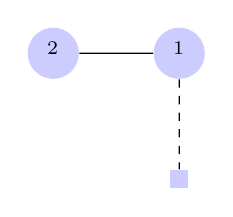
\begin{tikzpicture}
      [scale=.8,auto=left,every node/.style={circle,fill=blue!20}]
      \node (n1) at (3,3) {$\tehole^{1}$};
      \node (n2) at (1,3)  {$\tehole^{2}$};
      \node[rectangle] (i) at (3,1)  {$\tnum$};
    
      \foreach \from/\to in {n1/n2}
        \draw (\from) -- (\to);
       \foreach \from/\to in {n1/i}
        \draw[dashed] (\from) -- (\to);
    
    \end{tikzpicture}
  \caption{Graph of $C = \{ \tehole^{1} \approx \tnum, ~ \tehole^{1} \approx~ \tehole^{2}\}$}
  \label{fig:sub1}
\end{subfigure}
\begin{subfigure}{.49\textwidth}
  \centering
  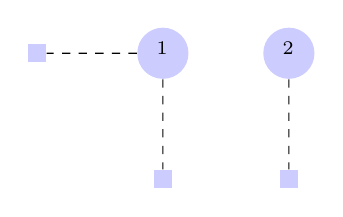
\begin{tikzpicture}
  [scale=.8,auto=left,every node/.style={circle,fill=blue!20}]
  \node (n1) at (2,3) {$\tehole^{1}$};
  \node (n2) at (4,3)  {$\tehole^{2}$};
  \node[rectangle] (i1) at (4,1)  {$\tnum$};
  \node[rectangle] (i2) at (2,1)  {$\tnum$};
  \node[rectangle] (i3) at (0,3)  {$\tbool$};

   \foreach \from/\to in {n1/i3, n1/i2, n2/i1}
    \draw[dashed] (\from) -- (\to);

\end{tikzpicture}
  \caption{Graph of $C = \{ \tehole^1 \approx \tnum, ~ \tehole^1 \approx \tbool, ~ \tnum \approx~ \tehole^2\}$}
  \label{fig:sub2}
\end{subfigure}
\caption{Sample constraint graphs of ground types}
\label{fig:ex1ex2graphs}
\end{figure}

Upon encountering a constraint between two arrow $\tarr{}{}$ types, the constraint solver generates a two new constraints on-the-fly: one between the left children of the arrows, and one between the right children of the arrows. For example, given the constraint set $C_{ex3} = \{ \tarr{\tehole^1}{\tehole^2} \approx \tarr{\tehole^3}{\tnum}$, the solver will generate $\tehole^1 \approx \tehole^3$ and $\tehole^2 \approx \tnum$. See Figure \ref{fig:arrowgraph} for the graph constructed from $C_{ex3}$. Note that the nodes $\tehole^1$ and $\tehole^3$ are \textit{linked} with a solid edge, but $\tehole^2$ is only \textit{tagged} with $\tnum$.

\begin{figure}[h!]
\centering
\begin{tikzpicture}[remember picture,
  inner/.style={circle,draw=blue!50,fill=blue!20,thick,inner sep=3pt},
  innerrect/.style={rectangle,draw=blue!50,fill=blue!20,thick,inner sep=3pt},
  outer/.style={draw=green,fill=green!20,thick,inner sep=10pt}
  ]
  \node[outer,draw=green] (A) {
    \shortstack{
        $Arrow$\\
        \begin{tikzpicture}
          \node [inner] (n1)  {$\tehole^{1}$};
          \node [inner,right=of n1] (n2) {$\tehole^{2}$};
          % \draw[red,thick,->] (n1) -- (n2);
        \end{tikzpicture}
    }
  };
  \node[outer,draw=green,below=of A] (B) {
    \shortstack{
        $Arrow$\\
        \begin{tikzpicture}
          \node [inner] (n3)  {$\tehole^{3}$};
          \node [innerrect,right=of n3] (i) {$\tnum$};
          % \draw[red,thick,->] (n3) -- (i);
        \end{tikzpicture}
    }
  };
  \draw (n1) -- (n3);
  \draw[dashed] (n2) -- (i);
   \draw[thick] (A) -- (B);
\end{tikzpicture}
\caption{Expanded constraint graph of $C_{ex3}$}
\label{fig:arrowgraph}
\end{figure}

We provide pseudocode for a graph construction algorithm in Figure \ref{fig:algcode_construct_graph}.  We assume a basic \emph{link\_nodes} and \emph{tag\_nodes} definition that connects nodes by retrieving a type hole's associated \emph{PotentialTypeSet} from the graph before extending it with some supplied type. We also assume the existence of a \emph{Map.add} function that adds a new element to the supplied map if it does not already exist, and otherwise does not change any values.

% A Union-Find implementation can use the following helper functions defined in \ref{fig:algcode_construct_graph_helpers}:
% \begin{enumerate}
%   \item add\_node() wraps an $Htyp$ in singleton PotentialTypeSet and adds it to the graph if not already present, and returns the updated graph.
%   \item link\_nodes() uses the Find operation of Union-Find to get the representatives of both nodes, then Unions both representatives, merging their \textit{PotentialTypeSet}s in the process as described in Figure \ref{fig:possible_type_sets}.
%   \item tag\_node() uses the Find operation of Union-Find to get the representative of a node, and adds $\tau$ to its \textit{PotentialTypeSet}.
% \end{enumerate}

% \begin{figure}[h!]
% \begin{lstlisting}[escapeinside={(*}{*)}]
% let link (graph, t1, t2) =
%     let s1 = graph.get(t1) in
%     let s2 = graph.get(t2) in
%     let s3 = s1 (*$\amalg$*) s2 in
%     let graph = graph.insert(t1, s3)in
%     let graph = graph.insert(t2, s3) in
%     graph;

% let tag (graph, t1, t2) =
%     let s = graph.get(t1) in
%     let s' = s (*$\amalg$*) single(t2) in
%     let graph = graph.insert(t1, s') in 
%     graph;
% \end{lstlisting}
% \vspace{-4px}
%  \hrule
% \caption{Algorithms for linking and tagging nodes in constraint graphs}
% \label{fig:algcode_link_tag}
% \end{figure}

\begin{figure}[h!]
\begin{lstlisting}[escapeinside={(*}{*)}]
let rec construct_graph (~graph=Map.empty(), constraints) =
    match constraints with
    | [] -> graph
    | hd::tl -> (
        match hd with
        | ((*$\tarr{t1_L}{t1_R}$*), (*$\tarr{t2_L}{t2_R}$*)) ->
            construct_graph(
                ~graph, 
                (((*$t1_L$*), (*$t2_L$*)))::(((*$t1_R$*), (*$t2_R$*)))::tl
            )
        | ((*$\tehole^{p}$*) as hole, t)
        | (t, (*$\tehole^{p}$*) as hole) ->
            let graph = Map.add(graph, hole, hole) in
            if (contains_hole(t)) then (
                let graph = Map.add(graph, t, t) in
                let graph = link_node(~graph, t, hole) in
                construct_graph(~graph, tl)
            ) else (
                let graph = tag(graph, hole, t) in
                construct_graph(~graph, tl)
            )
        | _ -> construct_graph(~graph, tl)
    );

\end{lstlisting}
\vspace{-4px}
\hrule
\caption{Constraint graph creation algorithm of type hole inference}
\label{fig:algcode_construct_graph}
\end{figure}

% When a constraint of the form $A \approx B$ is processed, both A and B's \textit{PotentialTypeSet}s are recovered from the graph and then \textit{link}ed. When computing connected components, the link operation may be adjusted to identify a single representative among $A$ and $B$ via union-find. This representative can then be updated with the union of $A$ and $B$'s \textit{PotentialTypeSet}s. As other \textit{link} operations are performed on $A$ or $B$, union-find allows us to update a single \textit{PotentialTypeSet} shared among all members of their known \textit{connected component}. In this manner, the \texit{PotentialTypeSet} associated with any representative can act as an accumulated connected component across the entirety of \textit{constructGraph}. The changes necessary to \textit{link} and \textit{tag} are shown below in Figure ~\ref{fig:algocode_construct_graph}.

The function construct\_graph builds a mapping from each type hole to a \emph{PotentialTypeSet} containing its adjacency list. This \textit{PotentialTypeSet} is only an adjacency list, a subset of the full solution for the type hole. A depth-first search can be used to determine all nodes in the graph which can be reached from a type hole using this adjacency list.

Alternatively, a Union-Find implementation can use the following definitions for these helper functions defined in \ref{fig:algcode_construct_graph_helpers}:
\begin{enumerate}
  \item add\_node() wraps an $Htyp$ in singleton PotentialTypeSet and adds it to the graph if not already present, and returns the updated graph.
  \item link\_nodes() uses the Find operation of Union-Find to get the representatives of both nodes, then Unions both representatives, merging their \textit{PotentialTypeSet}s in the process as described in Figure \ref{fig:possible_type_sets}.
  \item tag\_node() uses the Find operation of Union-Find to get the representative of a node, and adds $\tau$ to its \textit{PotentialTypeSet}.
\end{enumerate}
Using these helper functions, the graph returned by construct\_graph will contain the full \textit{PotentialTypeSet} for each type hole, not just an adjacency-list.

\begin{figure}[h!]
\begin{lstlisting}[escapeinside={(*}{*)}]
let add_node (graph, t) =
    graph.add(graph, t, [])
let link_nodes (graph, t1, t2) =
    let (rep1, rep2) = (UnionFind.find(t1), UnionFind.find(t2)) in
    let (s1, s2) = (graph.find(rep1), graph.find(rep2)) in
    let union_rep = UnionFind.union(rep1, rep2) in
    let s_merged = s1 (*$\amalg_{UF}$*) s2 in
    Map.update(graph, union_rep, s_merged)
let tag_node (graph, t1, t2) =
    let rep1 = UnionFind.find(t1) in
    let s = graph.get(rep1) in
    let s' = s (*$\amalg_{UF}$*) UnionFind.elem([t2]) in
    Map.update(graph, t1, s')
\end{lstlisting}
\vspace{-2px}
\hrule
\caption{Constraint solving algorithm helper functions, using Union-Find. Assumes the use of $\amalg_{UF}$ operation}
\label{fig:algcode_construct_graph_helpers}
\end{figure}

In order to accommodate this change while ensuring that the left and right children of $\tarr{}{}$ \textit{PotentialType}s are also merged properly, minor adjustments must be made to the definitions presented in Figure \ref{fig:possible_type_sets}. However, the definitions are somewhat redundant, and are consequently left to Appendix A for reference.

An additional step is taken to mark type holes with an error if they occur within their own \textit{PotentialTypeSet}. In Hindley-Milner type inference this is referred to as the occurs-check. In the context of \textit{PotentialTypeSet}s, this problem can be re-framed as determining if a \textit{PotentialTypeSet} has a cycle.

Type holes are considered solvable if their \textit{PotentialTypeSet} contains a single type. If a type hole's \textit{PotentialTypeSet} contains multiple, conflicting types, or contains no types, or if the type hole fails the occurs check, then it is considered unsolvable. In both cases, helpful visual feedback can be provided to the user.

% The end result of constraint solving is a mapping from every type hole to its \textit{PotentialTypeSet}. If the user has made no errors when writing their program, each type hole's \textit{PotentialTypeSet} should be acyclic and contain no conflicting ground types. However, if a program is incomplete or erroneous, the list of suggestions for a type hole may contain multiple types, which have all been constrained to the type hole at some point during constraint generation. The user can then inspect the set of type suggestions and assess which one is correct, and based on the incorrect types suggested, make corrections to the program.

\begin{figure}[h!]
\begin{lstlisting}[escapeinside={(*}{*)}]
let handle_occurs_check (graph) =
    // annotate solution with occurs check errors
    let annotate_with_error (key) =
        let s = Map.find(graph, UnionFind.find(key) in
        let pass_occurs = is_acyclic(s)
        (key, s, pass_occurs)
    in
    List.map(Map.keys(graph), annotate_with_error)
}
\end{lstlisting}
\vspace{-4px}
 \hrule
\caption{Constraint solving algorithm of type hole inference}
\label{fig:occurs_check}
\end{figure}

\subsection{Future Work}
\subsubsection{Other Binary Types and Parametric Polymorphism}
In order to extend our definitions of \emph{PotentialTypeSet}s to other binary types like $\tau_1 \times \tau_2$ or $\tau_1 + \tau_2$ and allow parametric polymorphism, we simply update our definitions of hole provenances and \emph{PotentialTypeSet}s as defined in Figure \ref{fig:extended_merging_possible_type_sets}

\todo{Discuss other needed provenances and matched rules}

\begin{figure}[h!]
\centering
$\arraycolsep=4pt\begin{array}{lll}
HProv~~ p & ::= & 
    n ~\vert~ 
    \rightarrow_{L}(p) ~\vert~ 
    \rightarrow_{R}(p) ~\vert~ 
    \times_{L}(p) ~\vert~ 
    \times_{R}(p) ~\vert~ 
    \mathtt{+}_{L}(p) ~\vert~ 
    \mathtt{+}_{R}(p)
    \\
HTyp~~ \tau & ::= &
  \tnum ~\vert~
  \tbool ~\vert~
  \tarr{\tau}{\tau} ~\vert~
  \tau_1 \times \tau_2 ~\vert~
  \tau_1 + \tau_2 ~\vert~
  \tehole^p
  \\
\end{array}$
\label{fig:syntax_possible_type_sets}
\caption{Extended syntax of HProv and HTyp}
\hrule
$\arraycolsep=4pt\begin{array}{lll}
BinaryOperator~~ \square & ::=~~~~~
\rightarrow  ~\vert~ 
\times  ~\vert~ 
\mathtt{+}
\\
PotentialTypeSet~~ s & = list(PotentialType)
\\
PotentialType~~ t & ::= 
  \tnum ~\vert~
  \tbool ~\vert~
  \TVar ~\vert~
  \tehole^p ~\vert~
  s ~\square~ s
  \\
\end{array}$
\label{fig:syntax_possible_type_sets}
\caption{Extended syntax of PotentialTypeSets and PotentialTypes}
\vspace{5px}
\hrule
\[\begin{array}{rcl}
    % base case: empty list
    s \amalg [] & = & s \\
    % both heads are the same, keep one
    \left[t,...s\right] ~\amalg~ \left[t,...s'\right] & = & \left[t,...s\right] ~\amalg~ s' \\
    % both heads are arrows, combine their children
    \left[s_L ~ \square_{\alpha} ~ s_R,...s_{tl}\right] ~\amalg~ \left[s'_L ~ \square_{\alpha} ~ s'_R,...s'_{tl}\right] & = & \left[(s_L ~\amalg~ s'_L) ~ \square_{\alpha} ~ (s'_R ~\amalg~ s'_R),...s_{tl}\right] ~\amalg~ s'_{tl} \\
    % both heads are different (but not arrows), keep both
    \left[t,...s\right] ~\amalg~ \left[t',...s'\right] & = & \left[t',t,...s\right] ~\amalg~ s' \\

    % old NeList version:
    % single(s_1 ~\square_{\alpha}~ s_2) ~\amalg~ single(s_3 ~\square_{\alpha}~ s_4) & = & single((s_1 ~\amalg~ s_3) ~\square_{\alpha}~ (s_2 ~\amalg~ s_4)) \\
    % single(t) ~\amalg~ single(t') & = & cons(t, single(t')) \\
    % cons(t,s) ~\amalg~ single(t) & = & cons(t, s) \\
    % cons(s_1 ~\square_{\alpha}~ s_2, s) ~\amalg~ single(s_3 ~\square_{\alpha}~ s_4) & = & cons((s_1 ~\amalg~ s_3) ~\square_{\alpha}~ (s_2 ~\amalg~ s_4), s) \\
    % cons(t,s) ~\amalg~ cons(t',s') & = & cons(t,s) ~\amalg~ single(t') ~\amalg~ s' \\
\end{array}\] 
\caption{Extended rules for merging PotentialTypeSets}
\vspace{5px} 
\hrule
\label{fig:extended_merging_possible_type_sets}
\vspace{-5px}
\end{figure}
Here, we take a more general approach to representing binary types. Namely, a \emph{PotentialType} may be the combination of two \emph{PotentialType}s through any \emph{BinaryOperator} $\square$. The rules for extension follow the same logic as before, where we enforce that extension of a \emph{PotentialTypeSet} containing $s_1 ~\square_{\alpha}~ s_2$ with $s_3 ~\square_{\alpha}~ s_4$ simply merges the left and right \emph{PotentialTypeSet}s, thus yielding $(s_1 ~\amalg~ s_3) ~\square_{\alpha}~ (s_2 ~\amalg~ s_4)$. Additionally, we choose to represent type variables as a ground type, thus enforcing that type variables are inconsistent with other ground types and consistent with type holes and each other. 

In a system with parametric polymorphism, one thing we may be tempted to do is generalize \emph{PossibleTypeSet}s containing only type holes to a new type variable. However, there are a few subtle issues to be cautious of when considering this extension. Consider the following simple program:

\begin{center}
    \begin{lstlisting}[escapeinside={(*}{*)}, xleftmargin=.2\textwidth, xrightmargin=.2\textwidth]
        let x : (*$?^1$*) = (*$\ehole^2$*) in x
    \end{lstlisting}
\end{center}

We can see that x is never constrained to any complete types. In fact, the only constraint in this program is that $?^1 \approx \tehole^2$. Suppose that we were to suggest the type variable \lstinline{'a} as a type hole filling for $?^1$ and the user accepted this suggestion. We'd end up with the following program:

\begin{center}
    \begin{lstlisting}[escapeinside={(*}{*)}, xleftmargin=.2\textwidth, xrightmargin=.2\textwidth]
        let x : 'a = (*$\ehole^2$*) in x
    \end{lstlisting}
\end{center}

However, we've run into a stark issue: the only possible expressions that can replace $\tehole^2$ are expressions that analyze against \lstinline{'a}! This is far from ideal: we can see in the initial program that the user didn't express any clear intention for $\tehole^2$ to be strictly polymorphic.

We generalize this notion and make the following observation: whenever the user creates expression holes, there are any number of potential "unknown" constraints that could spawn from the expression hole after it is filled. Indeed, rather than such expression holes being polymorphic, which would effectively represent a lack of constraints on type apart from other unconstrained polymorphic types, they can be constrained to $\mathtt{ANY}$ type after being filled. This status can be effectively represented in a new type of constraint: the $\mathtt{ANY}$ constraint. If a type hole $?^p$ is constrained to $\mathtt{ANY}$, it cannot be generalized to a type variable. On the other hand, if a type hole is never constrained to $\mathtt{ANY}$, it \emph{can} be generalized to a type hole. In order to concretize this notion and allow it to be represented in our constraint graph, we update rules 1f and 1g in Figure \ref{fig:ana-syn} as follows:

\begin{equation}
    \inferrule[]{ }{
        \consexptyp{\Gamma}{\llparenthesiscolor \rrparenthesiscolor^n}{\tehole^n}{\{ \tehole^n \approx \mathtt{ANY} \}}
      }
\end{equation}
\vspace{-3px}
\begin{equation}
    \inferrule[]{
        \consexptyp{\Gamma}{e}{\tau}{C}
       }{
         \consexptyp{\Gamma}{\llparenthesiscolor e \rrparenthesiscolor^n}{\tehole^n}{C \cup \{ \tehole^n \approx \mathtt{ANY} \}}
       }
\end{equation}
\\
These changes ensure that expression holes synthesize type holes that are constrained to the $\mathtt{ANY}$ type. These type holes and any other type holes constrained to them can never be generalized to type variables. The definition of \emph{PossibleType}s can also be adjusted slightly to account for this change:
\begin{center}
$\arraycolsep=4pt\begin{array}{lll}
PotentialType~~ t & ::= 
  \tnum ~\vert~
  \tbool ~\vert~
  \TVar ~\vert~
  \mathtt{ANY} ~\vert~
  \tehole^p ~\vert~
  s ~\square~ s
  \\
\end{array}$
\end{center}

\todo{solution when ANY with num and ANY with var}

\subsubsection{User Interaction and Conflict Highlighting}
To further the goal of helping users repair their programs, it would be beneficial to assign blame by highlighting the portions of the program responsible for the unsolved status of a \textit{PotentialTypeSet}. To allow this, constraints could be extended to contain the unique identifier of the expression from which they originated. Highlighting all expressions of the program which resulted in an unsolved \textit{PotentialTypeSet}, rather than attempting to localize the error to one particular expression, would result in less confusion and give the user more clues to discover the true source of a type error.
%These identifiers effectively act as reasons for edges within our constraint graph, enabling us to describe the exact series of reasons that caused the inference algorithm to conclude a type hole's solution status.



